\subsection{Simulations and discussion}
Through several tests, we have determined the following values to obtain acceptable results :
$$
\begin{cases}
    \xi = 0.8\\
    \omega_c = 5\\
    \alpha = 5
\end{cases}
$$
\subsubsection{Response to a reference variation}
The new reference has been set at \SI{0.002}{\meter} for simulations.
\begin{figure}[H]
    \centering
    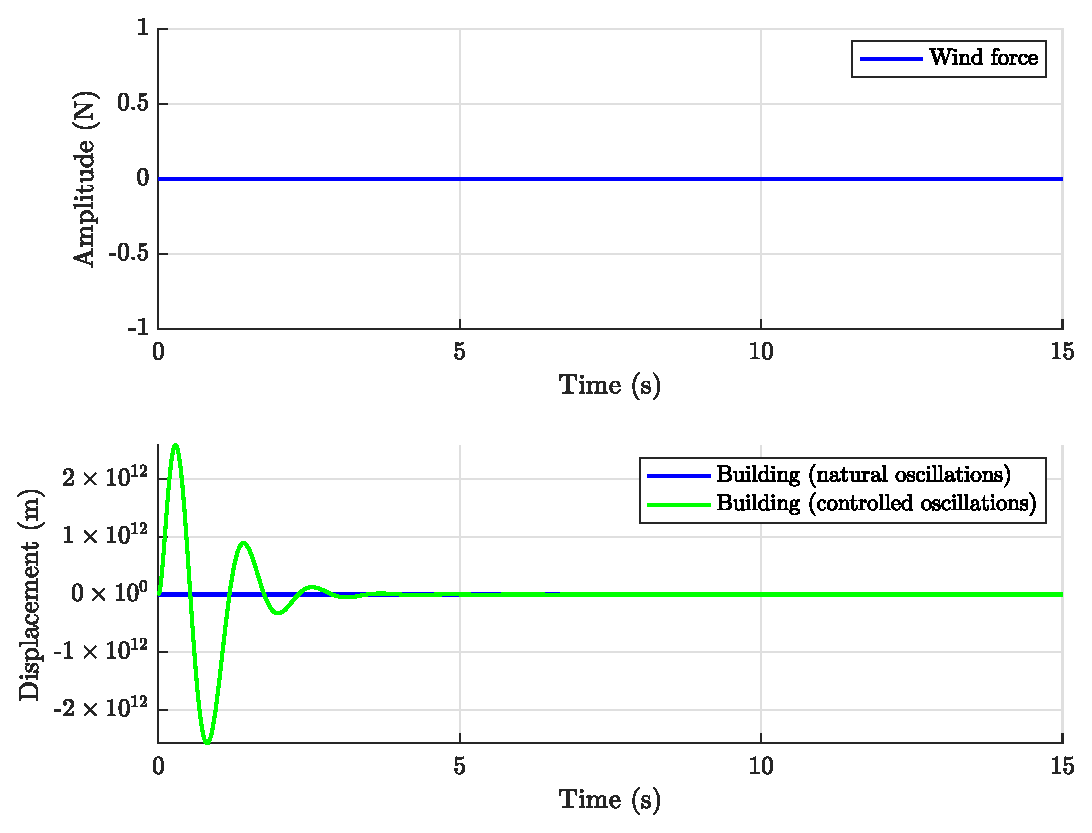
\includegraphics[width=\textwidth]{resources/eps/reference-controller.eps}
    \caption{Response to a reference variation - controlled output}
\end{figure}
\begin{figure}[H]
    \centering
    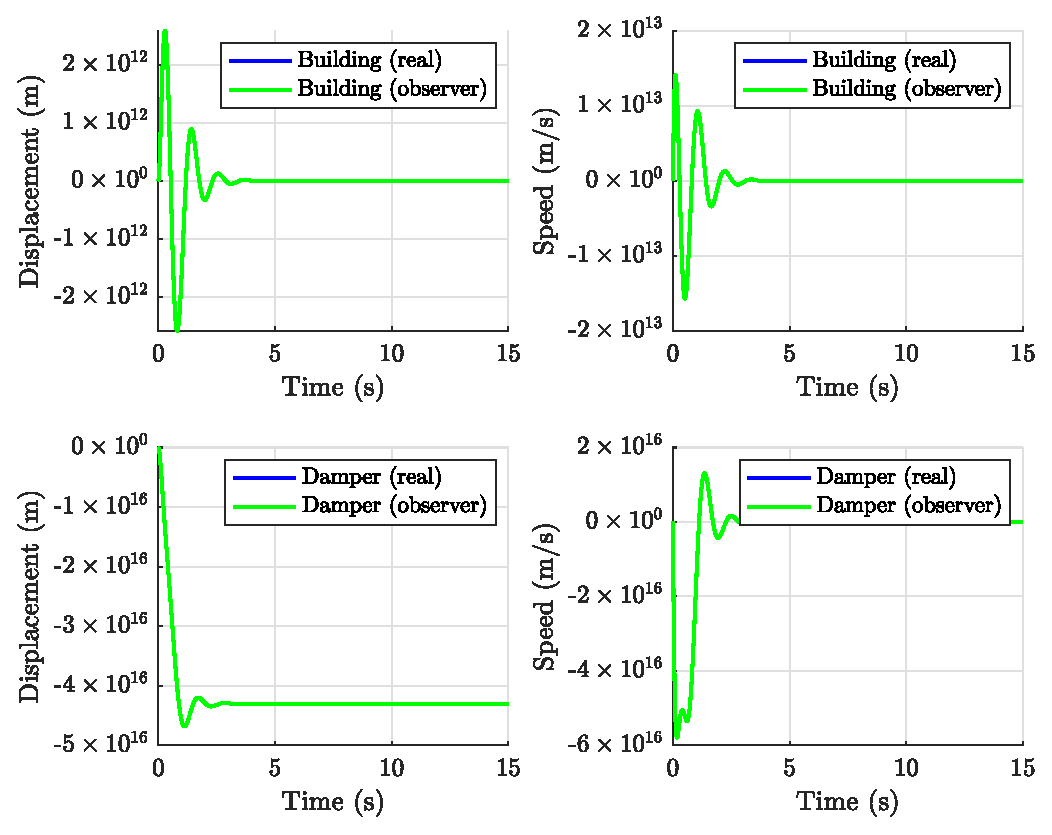
\includegraphics[width=\textwidth]{resources/eps/reference-observer.eps}
    \caption{Response to a reference variation - states}
\end{figure}

\subsubsection{Response to a perturbation (disturbance)}
For a constant wind force, we get : 
\begin{figure}[H]
    \centering
    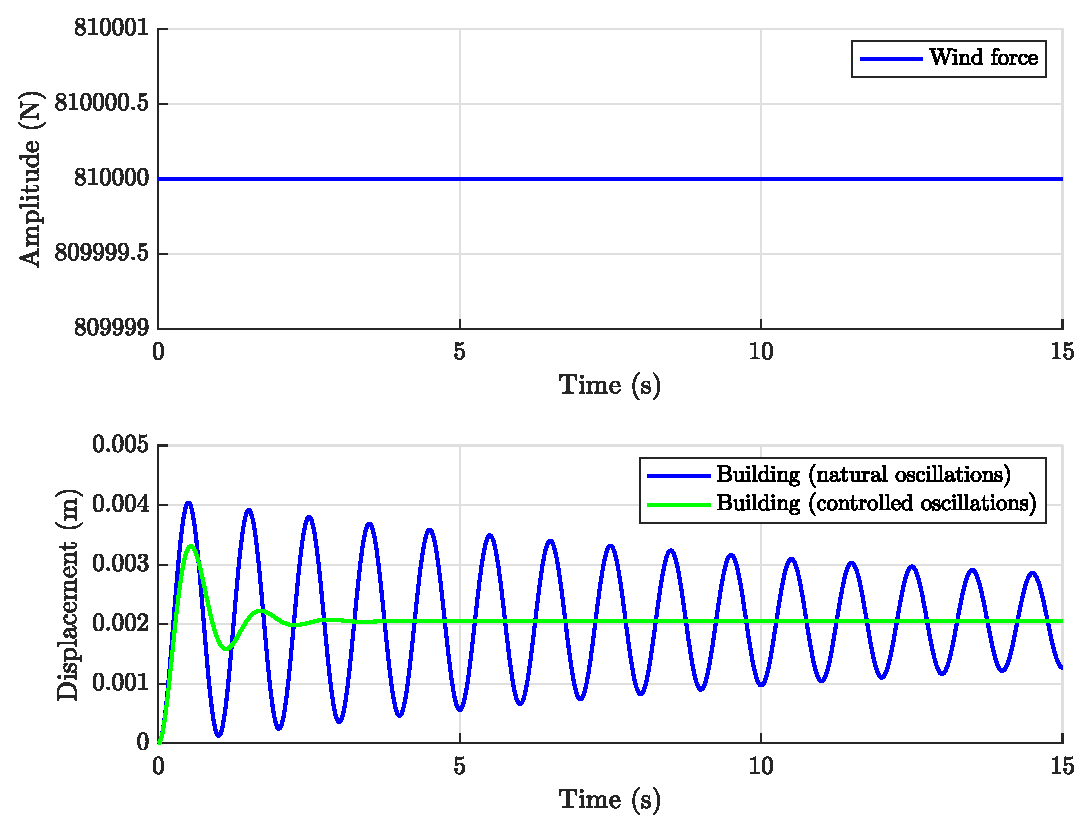
\includegraphics[width=\textwidth]{resources/eps/constant-controller.eps}
    \caption{Response to a constant wind force - controlled output}
\end{figure}
\begin{figure}[H]
    \centering
    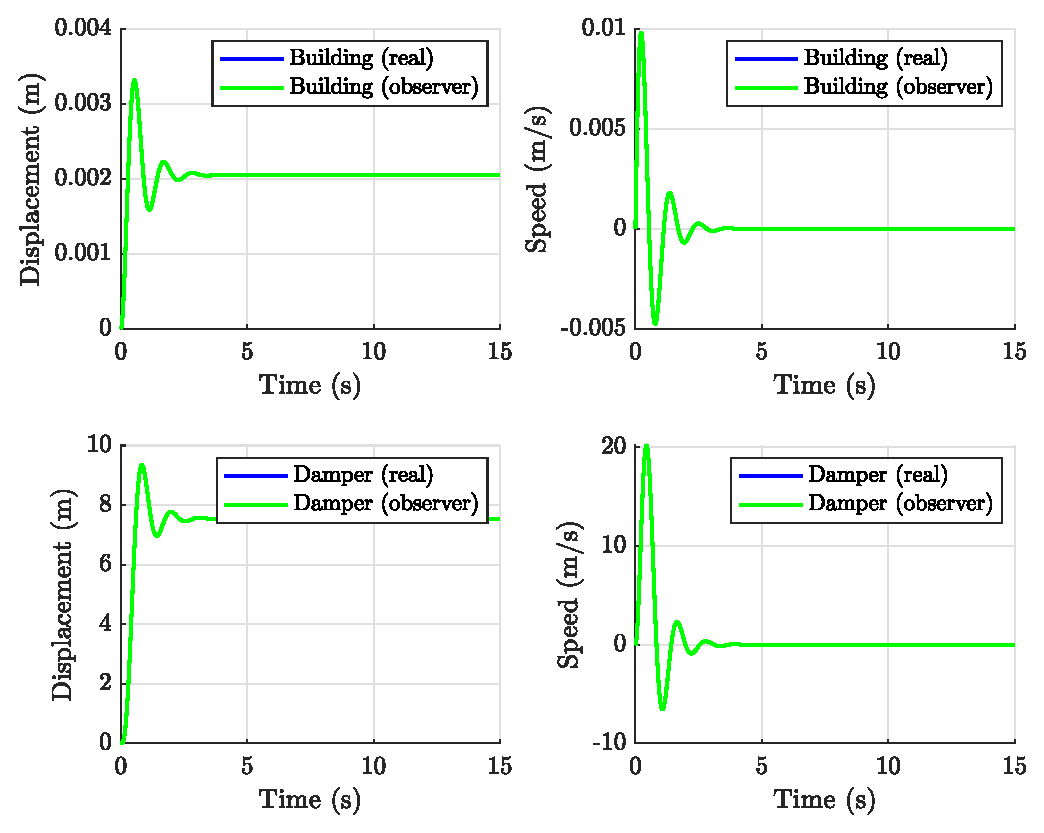
\includegraphics[width=\textwidth]{resources/eps/constant-observer.eps}
    \caption{Response to a constant wind force - states}
\end{figure}
For a sinusoidal wind force, we get : 
\begin{figure}[H]
    \centering
    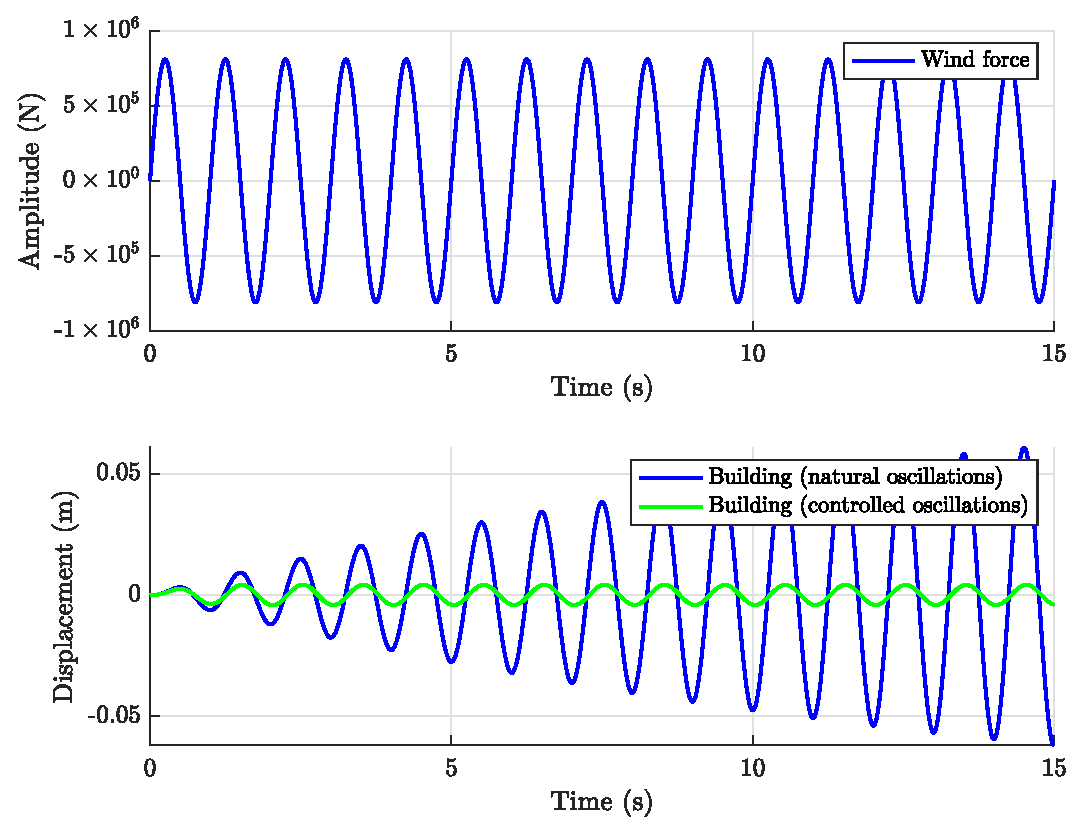
\includegraphics[width=\textwidth]{resources/eps/sinusoidal-controller.eps}
    \caption{Response to a sinusoidal wind force - controlled output}
\end{figure}
\begin{figure}[H]
    \centering
    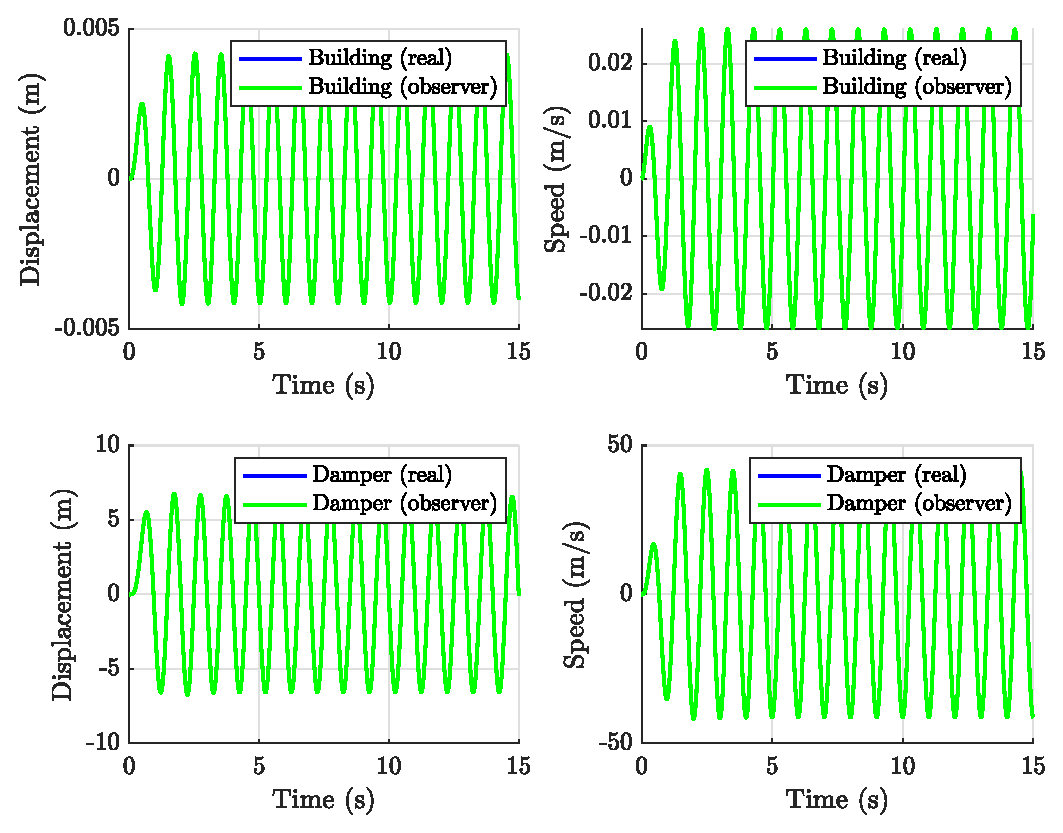
\includegraphics[width=\textwidth]{resources/eps/sinusoidal-observer.eps}
    \caption{Response to a sinusoidal wind force - states}
\end{figure}

\subsubsection{Presence of noise}
to do

\subsubsection{Impact of delays}
to do
